\documentclass[a4paper,12pt]{article}
\usepackage[utf8]{inputenc}
\usepackage{graphicx}
\usepackage{todonotes}
\usepackage{cite}

\begin{document}

\title{Bi-weekly activity report}
\maketitle
I would like to keep the structure of the report as it is in the following, since it is mostly to enforce a commitment on me. However if you would like me to include the full texts I can do so. I would expect that in the coming weeks the content will be more extensive as I had to do a lot more catching up on details I had forgotten than I expected.\\
I will send the next report in two weeks, most likely on the 15th.\\
If you have any suggestions towards the format or would like me to include full scale texts please let me know.

\section{Writing}
	Introductory texts concerning the following topics:
	\begin{enumerate}
		\item Systems code PROCESS for motivation of finding surrogate models.\\
		\item Basics of Bayesian statistics used in the GOGAP algorithm, currently in the appendix\\
		\item Brief descriptions of varying machine learning methods including Random forests, SVMs and boosting. Started on texts describing neural networks.
		\item Started working on descriptions of fusion devices. This needs more work the coming days since it is also referenced to by the PROCESS text and basis for parts in the model description section.
	\end{enumerate}

\section{Data Analysis}
	Sadly not as much as I wanted to since I forgot more than I thought and needed to do more reading as a result.
	I have plotted the parameters against sputter rate as discussed, but most have an uniform distribution. Only a few parameters deviate from this behaviour. I have included two of the three plots with non uniform distributions in the following graphics \ref{P5N} and \ref{P6N}:\\
		\begin{figure}
			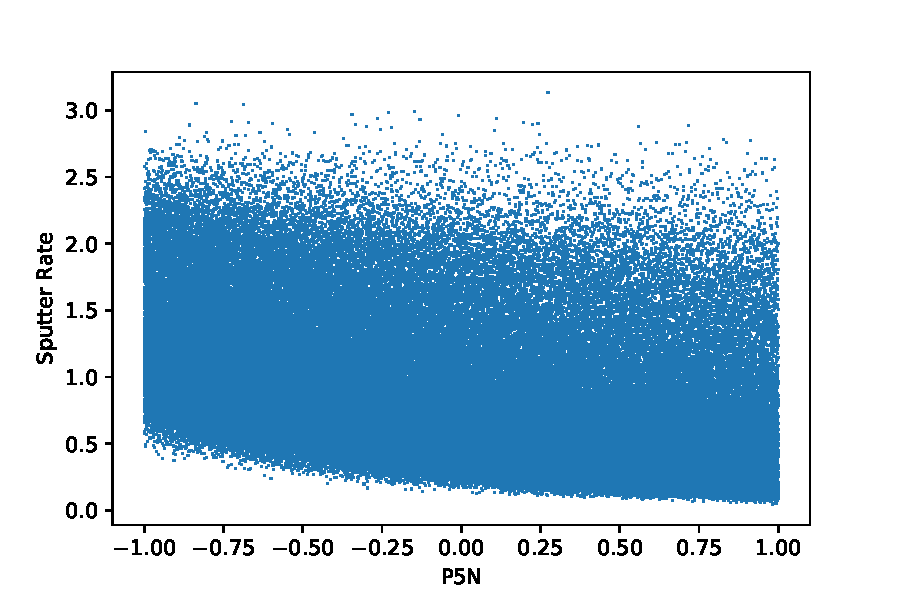
\includegraphics[width=0.8\textwidth]{../Thesis/images/P5N.pdf}
			\caption{Input parameter with non uniform sputter rate distribution: Plasma density at beginning of SOL}
			\label{P5N}
		\end{figure}
		\begin{figure}
			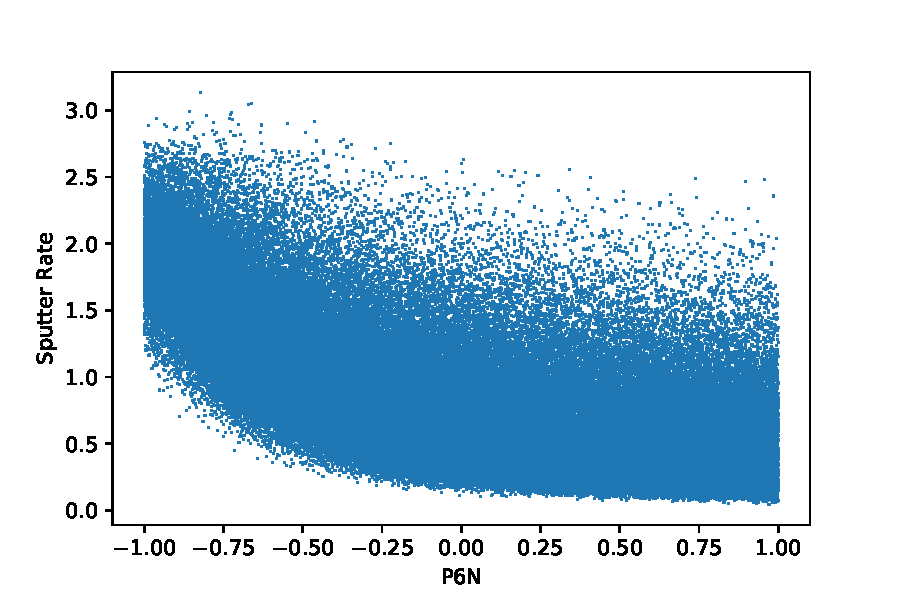
\includegraphics[width=0.8\textwidth]{../Thesis/images/P6N.pdf}
			\caption{Input parameter with non uniform sputter rate distribution: Plasma density at diverter / end of SOL}
			\label{P6N}
		\end{figure}
	~\\
	Please note that the Input parameters are plotted on a relative scale from $-1$ to $1$ within the given boundaries of the simulation parameters. They are not scaled to physical properties. The third parameter that has non uniform sputter rate distribution is also from the density profile, but has an even weaker trend than the one seen in fig. \ref{P5N}. I have not included the graph since it contains relativly large amounts of data with no new information.
\section{Additional Sources}
	No new sources added but reread many, including PhD Thesis from Mitja Beckers, basics of Bayesian statistics, stangeby for plasma physics and paper on PROCESS
\appendix
\end{document}